\documentclass[a4paper,12pt]{article}

\usepackage[T1]{fontenc}
\usepackage[utf8]{inputenc}
\usepackage{amsmath}
\usepackage{array}
\usepackage{booktabs}
\usepackage{caption}
\usepackage{float}
\usepackage{geometry}
\usepackage{graphicx}
\usepackage{hyperref}
\usepackage{setspace}
\geometry{margin=1in}
\setstretch{1.25}

\title{
    \vspace{-1.0cm}
    
\includegraphics[width=0.48\textwidth]{logo_hkust2.png}\\[0.8cm]
    \textbf{\Large Machine-Learning-Assisted Analysis and Optimization of a PSA CO$_2$ Capture Process}\\[0.4cm]
    \large SEEN5320 Final Project
}
\author{Your Name}
\date{\today}

\begin{document}
\maketitle

\begin{abstract}
This project integrates machine learning with a pressure swing adsorption (PSA) simulation dataset for CO$_2$ capture. A Latin Hypercube Sampling (LHS) design generated 1000 successful PSA operating cases. For each case, the last-cycle spatiotemporal profiles of pressure, gas composition, adsorbed loadings, gas temperature, and wall temperature were stored. The project converts those profiles into 470 physics-informed features, trains supervised surrogate models for purity, recovery, productivity, and energy, classifies high-performance cases, and uses PCA/K-means clustering to identify operating regimes. The best regression surrogate used design plus profile features and achieved a mean test $R^2$ of 0.982 across the four targets. The best high-performance classifier achieved an F1 score of 0.976. The analysis shows a strong purity--recovery conflict and identifies the light-product reflux ratio and late-step outlet profile features as the most influential predictors.
\end{abstract}

\tableofcontents
\newpage

\section{Objective and Research Question}
The objective is to use course-level machine learning methods to enhance interpretation and optimization of a PSA process simulation. The central research question is:

\begin{quote}
Can machine learning transform a 1000-sample LHS PSA simulation dataset and its final-cycle spatiotemporal profiles into accurate surrogates and interpretable operating insights?
\end{quote}

The project is designed around three tasks: predicting PSA performance without rerunning the mechanistic simulator, classifying promising operating cases, and explaining how design variables and final-cycle profiles connect to performance tradeoffs.

\section{Background and Literature Context}
PSA is widely used for gas separation because cyclic pressure changes can exploit adsorption selectivity without requiring a continuous solvent regeneration loop. For CO$_2$/N$_2$ separation, however, purity, recovery, productivity, and energy consumption are tightly coupled. Improving one objective can degrade another, especially when reflux and blowdown choices change where the CO$_2$ front sits inside the bed at the end of a cycle.

Classical PSA design relies on mechanistic cycle simulation and multi-objective search, building on adsorption process fundamentals \cite{ruthven1984adsorption}. This is physically meaningful but computationally expensive when many operating variables and cycle steps are explored. LHS is an established way to cover a simulation design space efficiently \cite{mckay1979lhs}. Machine learning offers a complementary route: regression models can approximate simulator outputs, classifiers can screen promising operating windows, and clustering/PCA can reveal regimes that are not obvious from a few scalar KPIs. The models used here connect to standard supervised-learning methods including random forests \cite{breiman2001random}, support vector machines \cite{cortes1995svm}, and neural-network regression \cite{bishop2006pattern}. This project therefore treats the simulator as the source of reliable labels and uses ML to extract reusable structure from the completed simulation campaign.

\section{Data and Feature Engineering}
\subsection{Simulation Dataset}
The dataset contains 1000 successful samples. Each row in \texttt{data/manifest.csv} contains seven LHS design variables and four performance metrics. The adsorbent is Zeolite 13X, and the PSA cycle includes co-current pressurization, adsorption, heavy reflux, co-current depressurization, counter-current depressurization, and light reflux steps.

\begin{table}[H]
\centering
\caption{LHS design variables used as ML inputs.}
\begin{tabular}{lll}
\toprule
Symbol & Meaning & Sampling range \\
\midrule
$x_1$ & Adsorption pressure & 100000--1000000 Pa \\
$x_2$ & Adsorption time & 10--5000 s \\
$x_3$ & Light-product reflux ratio & 0--1 \\
$x_4$ & Feed velocity & 0.1--1.0 m/s \\
$x_5$ & Blowdown pressure & 10000--100000 Pa \\
$x_6$ & Pressurization time & 0--100 s \\
$x_7$ & Counter-current depressurization time & 0--100 s \\
\bottomrule
\end{tabular}
\end{table}

The target outputs are CO$_2$ purity, CO$_2$ recovery, productivity in mol kg$^{-1}$ h$^{-1}$, and specific energy in kWh ton$^{-1}$. Energy was modeled as $\log_{10}(\mathrm{energy})$ during regression to reduce the influence of extreme high-energy cases.

\subsection{Profile Features}
For every sample, the final-cycle profile CSV stores values over time and axial bed position. The feature extraction script computes per-step means, ranges, standard deviations, final-step inlet and outlet values, final axial gradients, loading selectivity proxies, and gas-wall thermal lags for pressure, gas-phase CO$_2$, CO$_2$/N$_2$ loadings, gas temperature, and wall temperature. This produces 470 profile-derived features per sample and is saved as \texttt{data/profile\_features.csv}.

\begin{figure}[H]
\centering
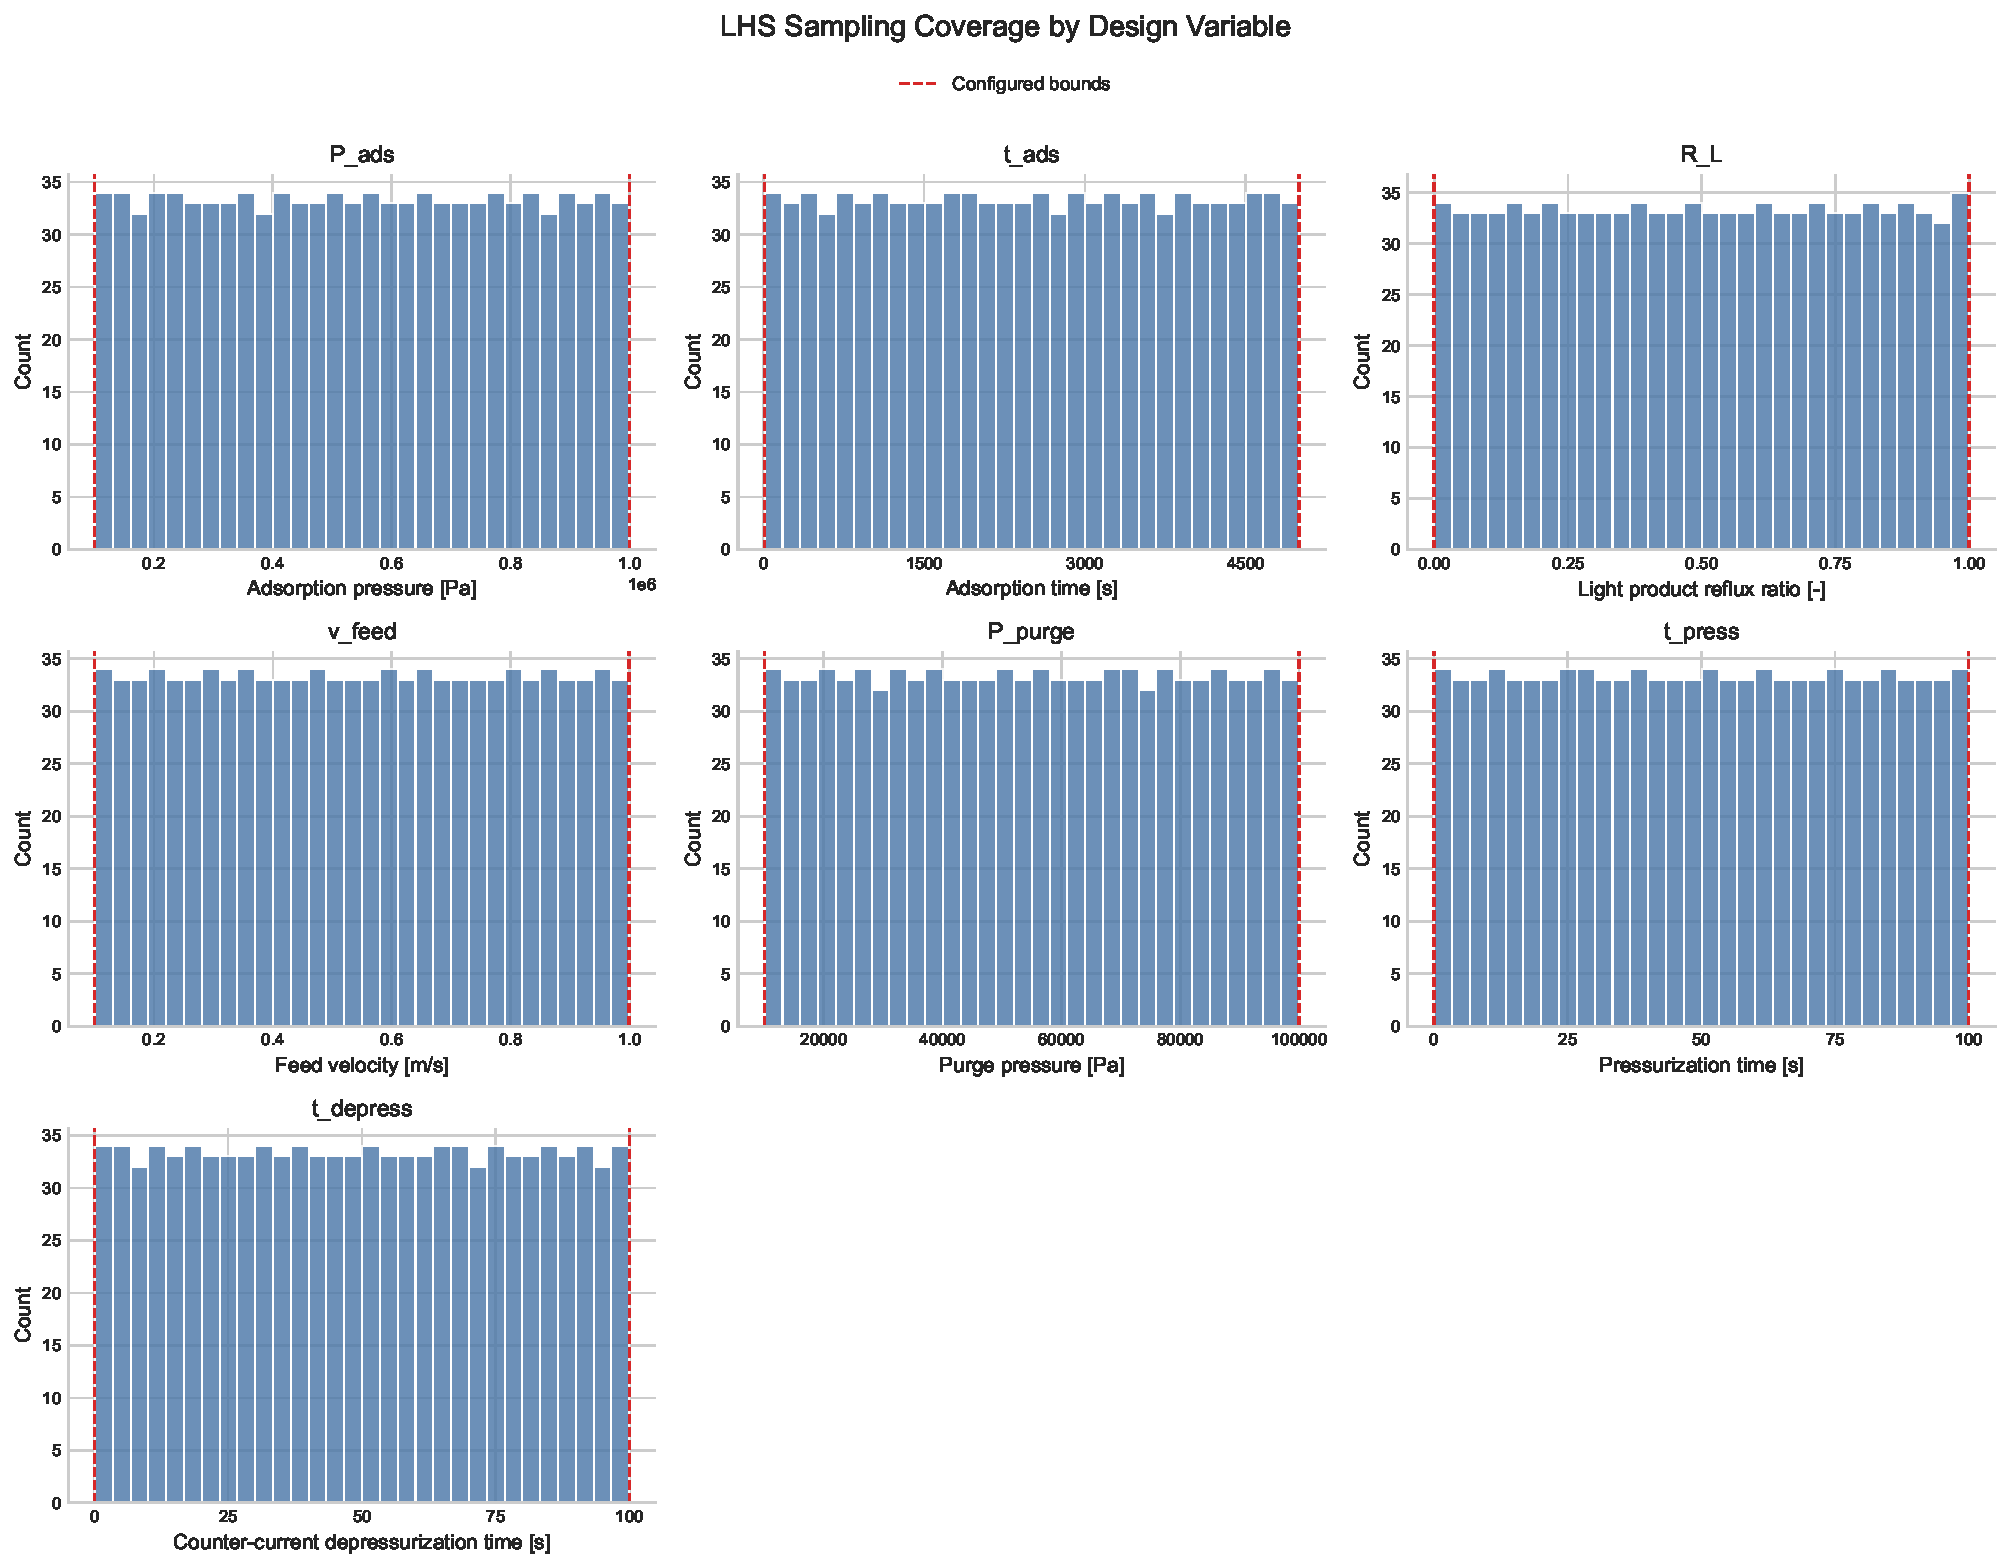
\includegraphics[width=0.92\textwidth]{figures/psa_manifest/01_sampling_coverage_histograms.pdf}
\caption{LHS coverage of the seven operating variables.}
\end{figure}

\section{Machine Learning Methodology}
The supervised regression task predicts purity, recovery, productivity, and log energy. Five regressors were evaluated: Ridge regression, random forest, gradient boosting, support vector regression, and a multilayer perceptron. Each was trained on two feature sets: design variables only, and design variables plus profile features. A fixed 80/20 train-test split with random seed 42 was used.

The classification task labels the top 20\% of samples by a balanced score:
\[
S = \frac{1}{4}\left[
\hat{p} + \hat{r} + \widehat{\mathrm{prod}} + \left(1-\widehat{\log_{10} E}\right)
\right],
\]
where hats denote min-max normalized values, $p$ is purity, $r$ is recovery, and $E$ is specific energy. Logistic regression, SVM, and random forest classifiers were compared.

For unsupervised analysis, PCA projects the combined design, KPI, and profile feature space into two dimensions, and K-means identifies four operating regimes. Pareto samples were computed using four objectives: maximize purity, recovery, and productivity, and minimize energy.

\section{Results and Discussion}
\subsection{Performance Tradeoffs}
The LHS campaign reveals a strong purity--recovery conflict with Spearman correlation $-0.691$. There are 138 four-objective Pareto samples. The highest-purity case reaches purity 0.670, but its recovery is only 0.0056 and its energy is 84379 kWh ton$^{-1}$. In contrast, the best balanced-score case keeps recovery near 0.996 and productivity near 106.6 mol kg$^{-1}$ h$^{-1}$, but purity remains close to the inlet CO$_2$ fraction. This is an important negative result: within the sampled region, high productivity and high recovery do not automatically imply meaningful CO$_2$ enrichment.

\begin{figure}[H]
\centering
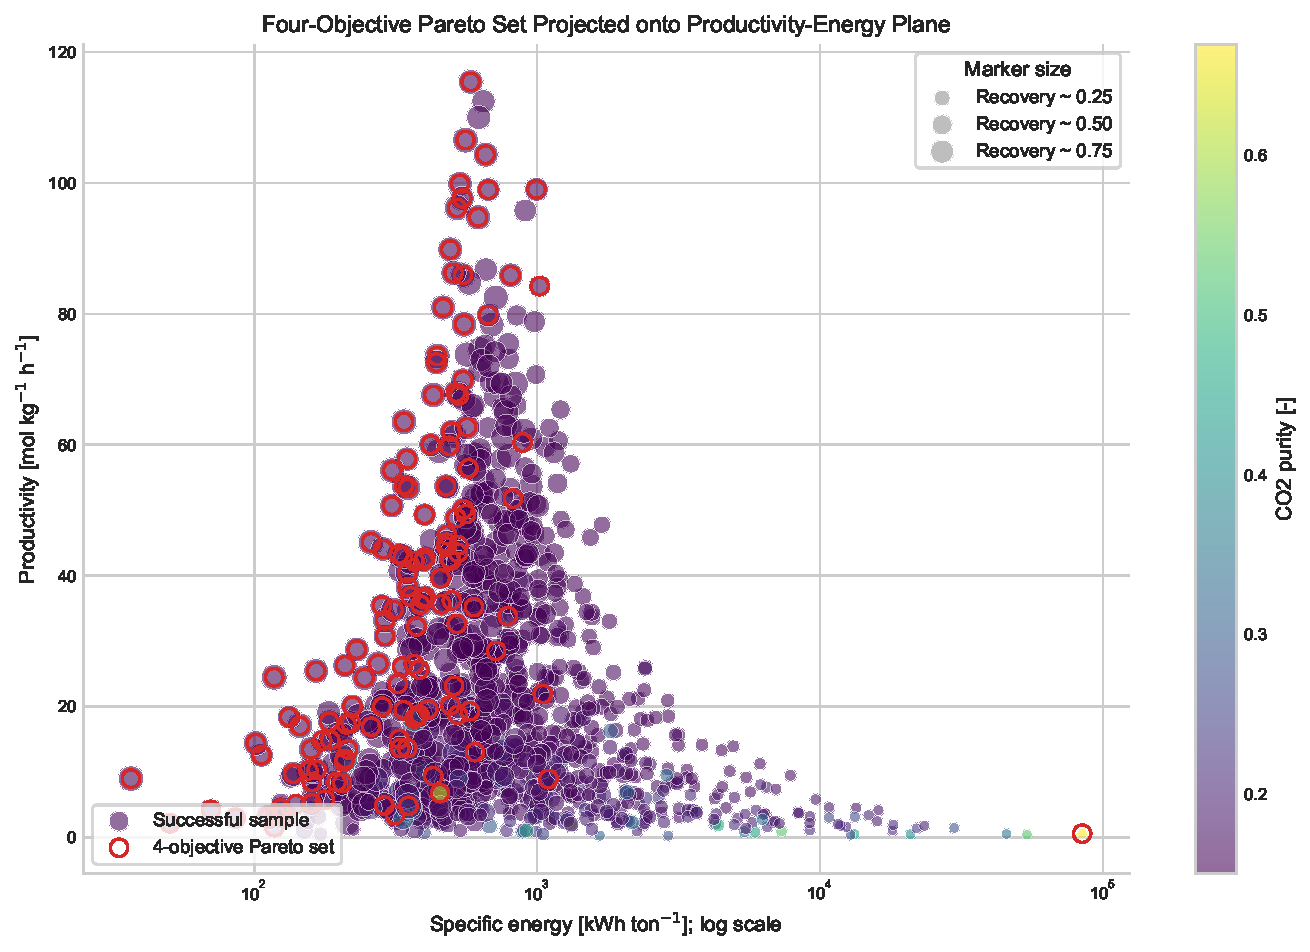
\includegraphics[width=0.92\textwidth]{figures/psa_manifest/04_objective_tradeoff_pareto.pdf}
\caption{Four-objective Pareto samples projected onto productivity and specific energy.}
\end{figure}

\subsection{Surrogate Model Accuracy}
Using only the seven design variables is useful, but adding final-cycle profile features substantially improves accuracy. The best model is Ridge regression with design plus profile features, achieving a mean test $R^2$ of 0.982. Per-target results are shown in Table \ref{tab:regression}.

\begin{table}[H]
\centering
\caption{Best regression surrogate performance on the 20\% test set.}
\label{tab:regression}
\begin{tabular}{lrrr}
\toprule
Target & RMSE & MAE & $R^2$ \\
\midrule
Purity & 0.00590 & 0.00356 & 0.98495 \\
Recovery & 0.00935 & 0.00491 & 0.99892 \\
Productivity & 1.70329 & 1.04535 & 0.99357 \\
$\log_{10}$(energy) & 0.08965 & 0.05600 & 0.95237 \\
\bottomrule
\end{tabular}
\end{table}

\begin{figure}[H]
\centering
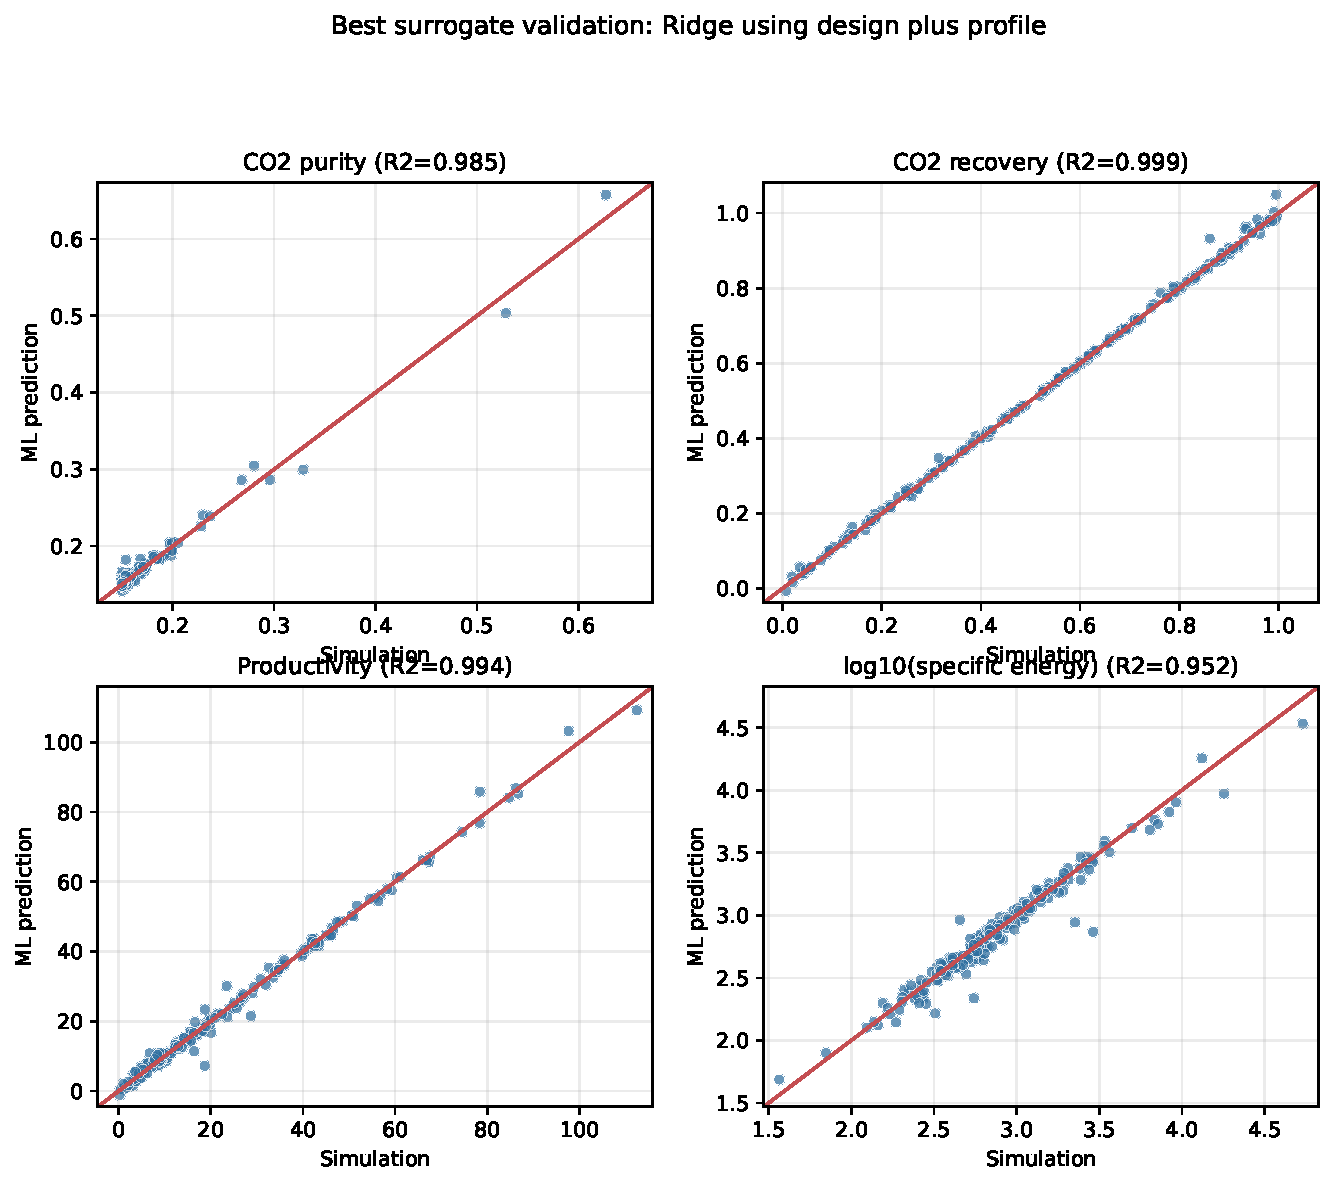
\includegraphics[width=0.92\textwidth]{figures/psa_ml/01_regression_predicted_vs_simulated.pdf}
\caption{Predicted versus simulated targets for the best surrogate.}
\end{figure}

\begin{figure}[H]
\centering
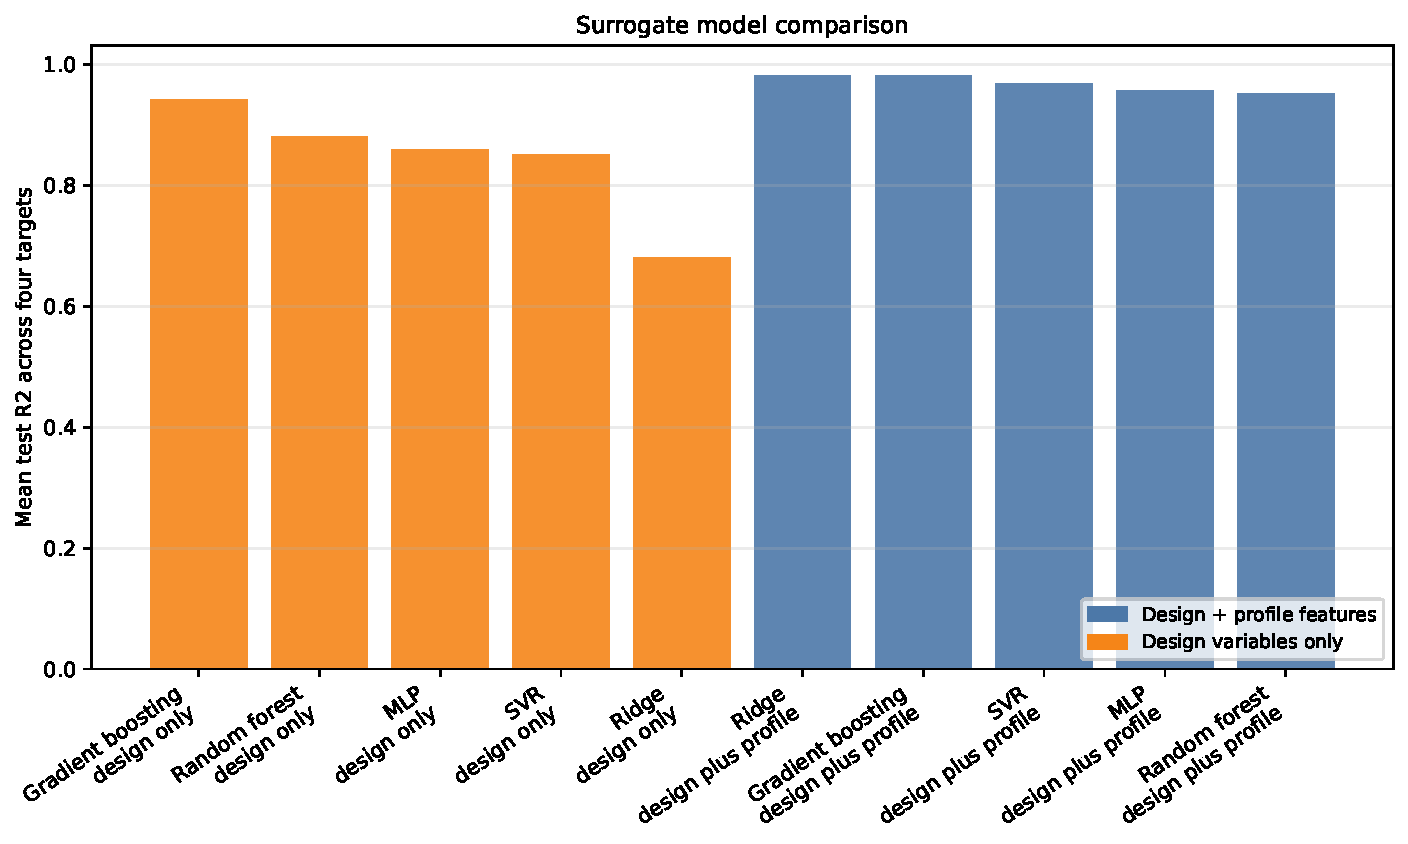
\includegraphics[width=0.88\textwidth]{figures/psa_ml/02_model_metric_comparison.pdf}
\caption{Regression model comparison. Profile features consistently improve test-set accuracy.}
\end{figure}

\subsection{High-Performance Classification}
The top 20\% balanced-score samples are treated as high-performance screening targets. Logistic regression is the best classifier, with accuracy 0.990, F1 score 0.976, and ROC-AUC 0.9995. This suggests that the high-performance region is separable once profile-informed features are included.

\begin{table}[H]
\centering
\caption{High-performance classification results.}
\begin{tabular}{lrrrrr}
\toprule
Model & Accuracy & Precision & Recall & F1 & ROC-AUC \\
\midrule
Logistic regression & 0.990 & 0.952 & 1.000 & 0.976 & 0.9995 \\
Random forest & 0.950 & 0.941 & 0.800 & 0.865 & 0.9903 \\
SVM & 0.925 & 0.736 & 0.975 & 0.839 & 0.9816 \\
\bottomrule
\end{tabular}
\end{table}

\begin{figure}[H]
\centering
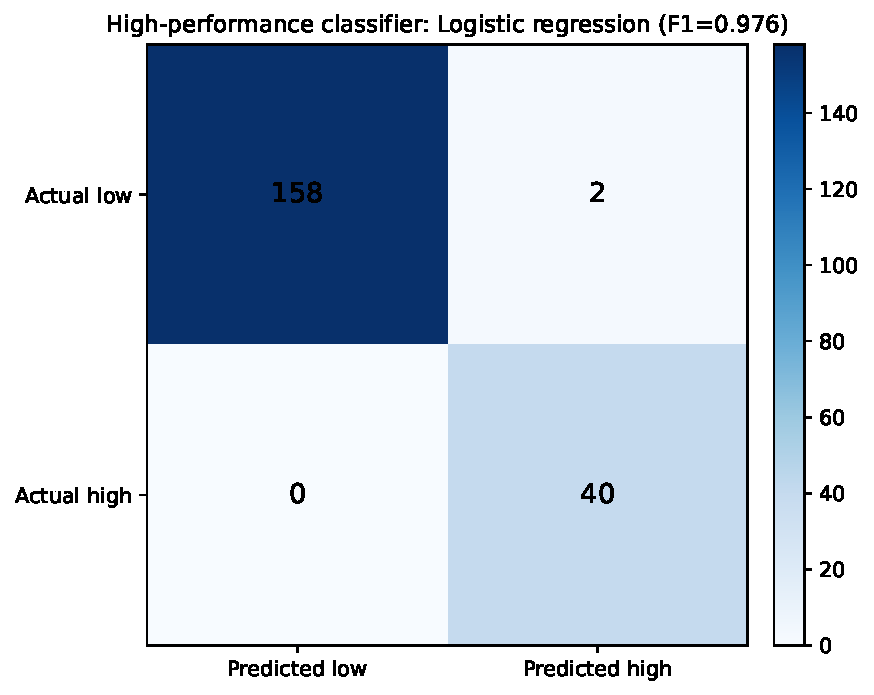
\includegraphics[width=0.55\textwidth]{figures/psa_ml/05_classification_confusion_matrix.pdf}
\caption{Confusion matrix for the best high-performance classifier.}
\end{figure}

\subsection{Interpretability and Operating Regimes}
Random forest feature importance identifies the light-product reflux ratio $x_3$ as the dominant input. Several light-reflux-step outlet features are also important, including outlet gas temperature, outlet pressure, and final axial pressure and CO$_2$ gradients. This aligns with PSA intuition: reflux and late-cycle regeneration determine how much CO$_2$ remains in the bed and therefore shape the purity--recovery tradeoff.

\begin{figure}[H]
\centering
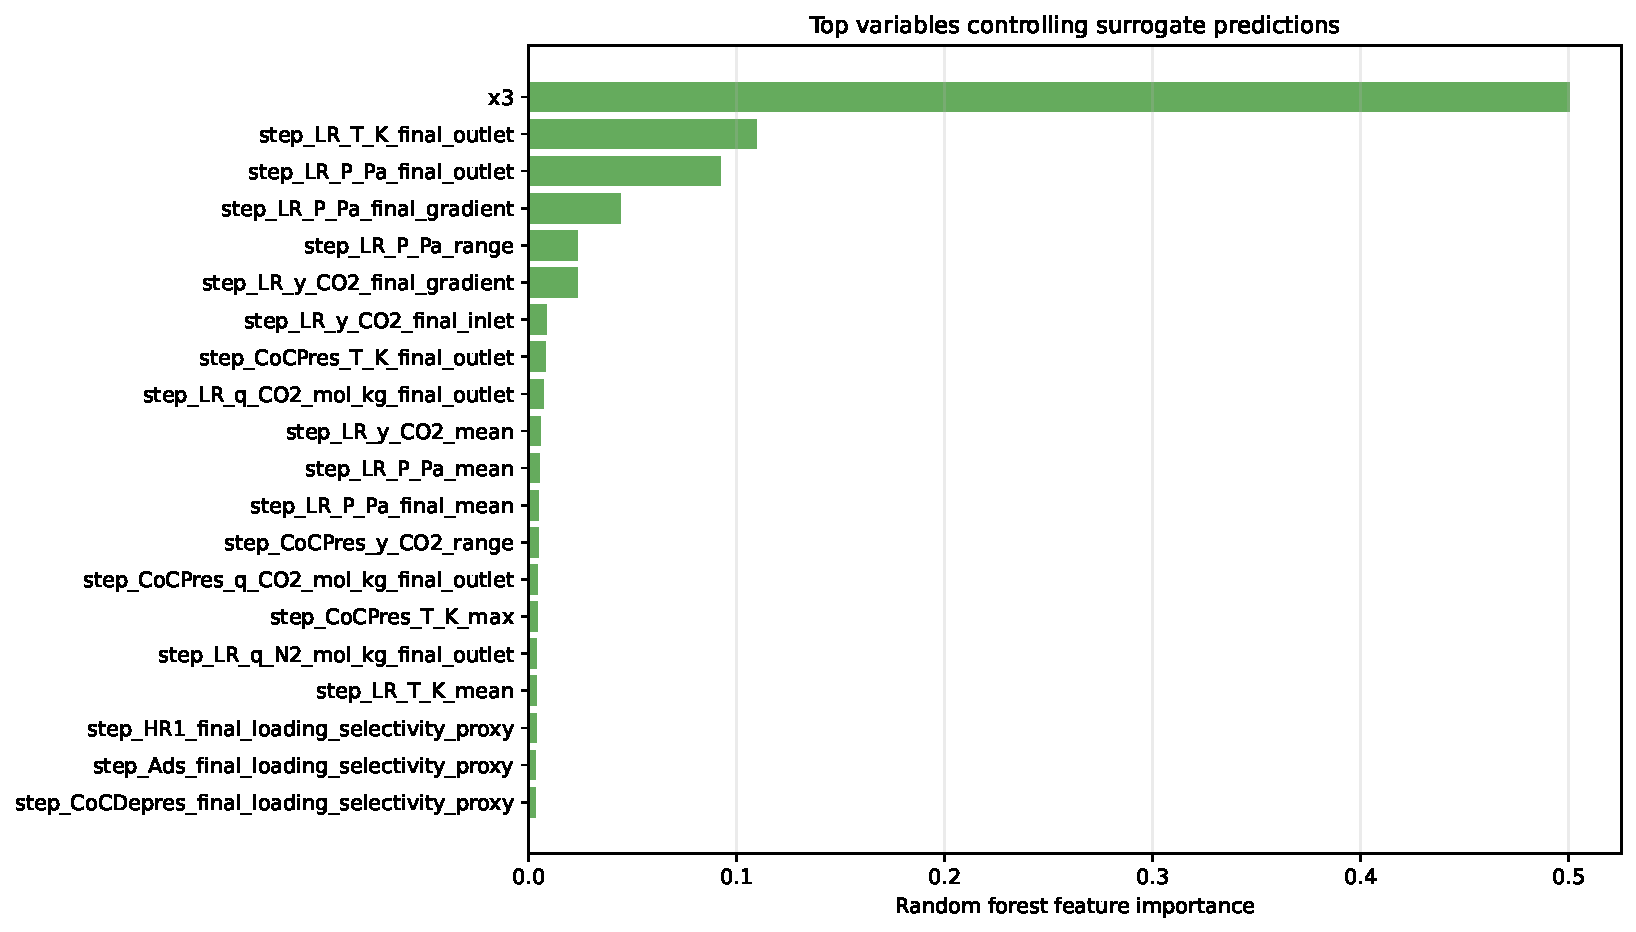
\includegraphics[width=0.88\textwidth]{figures/psa_ml/03_feature_importance.pdf}
\caption{Top feature importances from the random forest surrogate.}
\end{figure}

The PCA/K-means map separates the operating space into regimes with different KPI patterns. Most samples occupy broad low-to-medium performance regions, while small high-recovery pockets appear as distinct groups. The adsorption-step heatmaps show that representative operating points have visibly different CO$_2$ fronts, reinforcing why profile features improve the surrogate.

\begin{figure}[H]
\centering
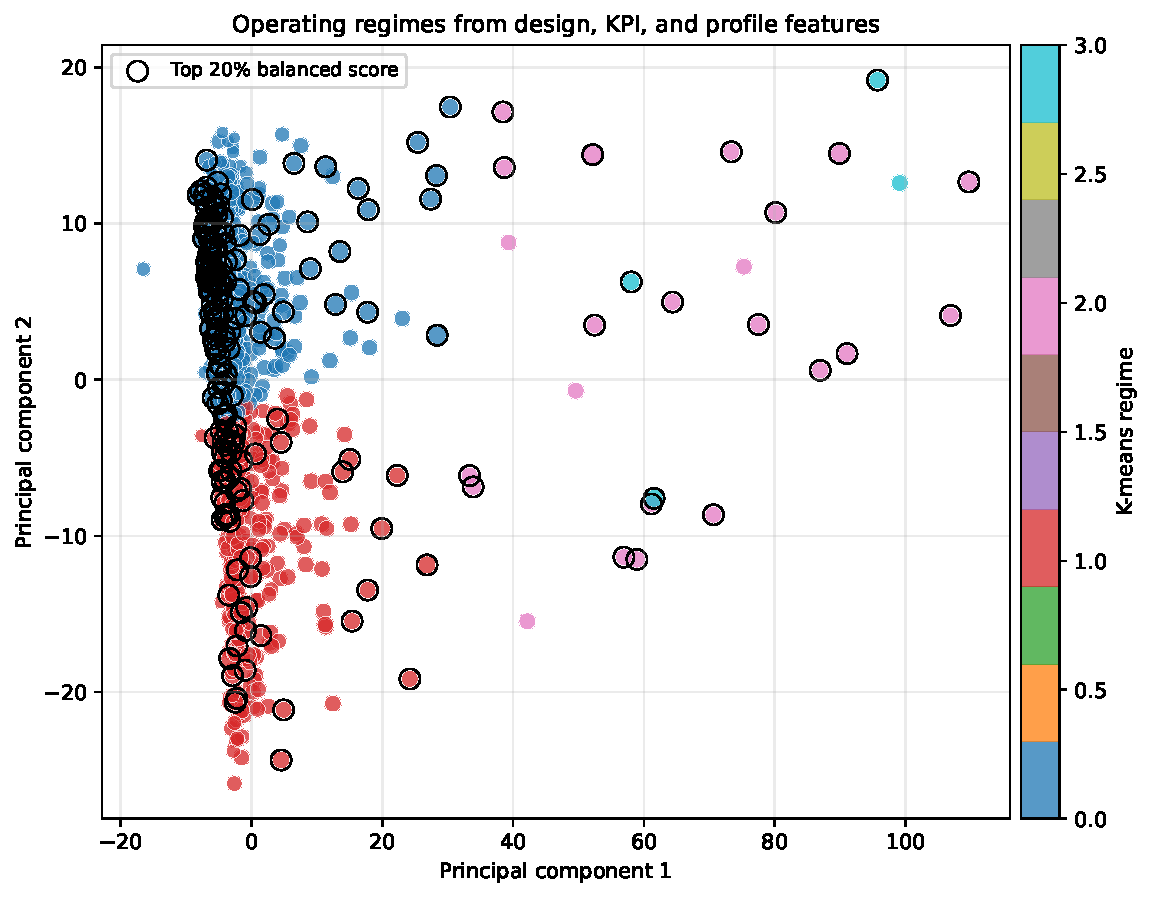
\includegraphics[width=0.80\textwidth]{figures/psa_ml/04_pca_operating_regimes.pdf}
\caption{Operating regimes from PCA and K-means clustering.}
\end{figure}

\begin{figure}[H]
\centering
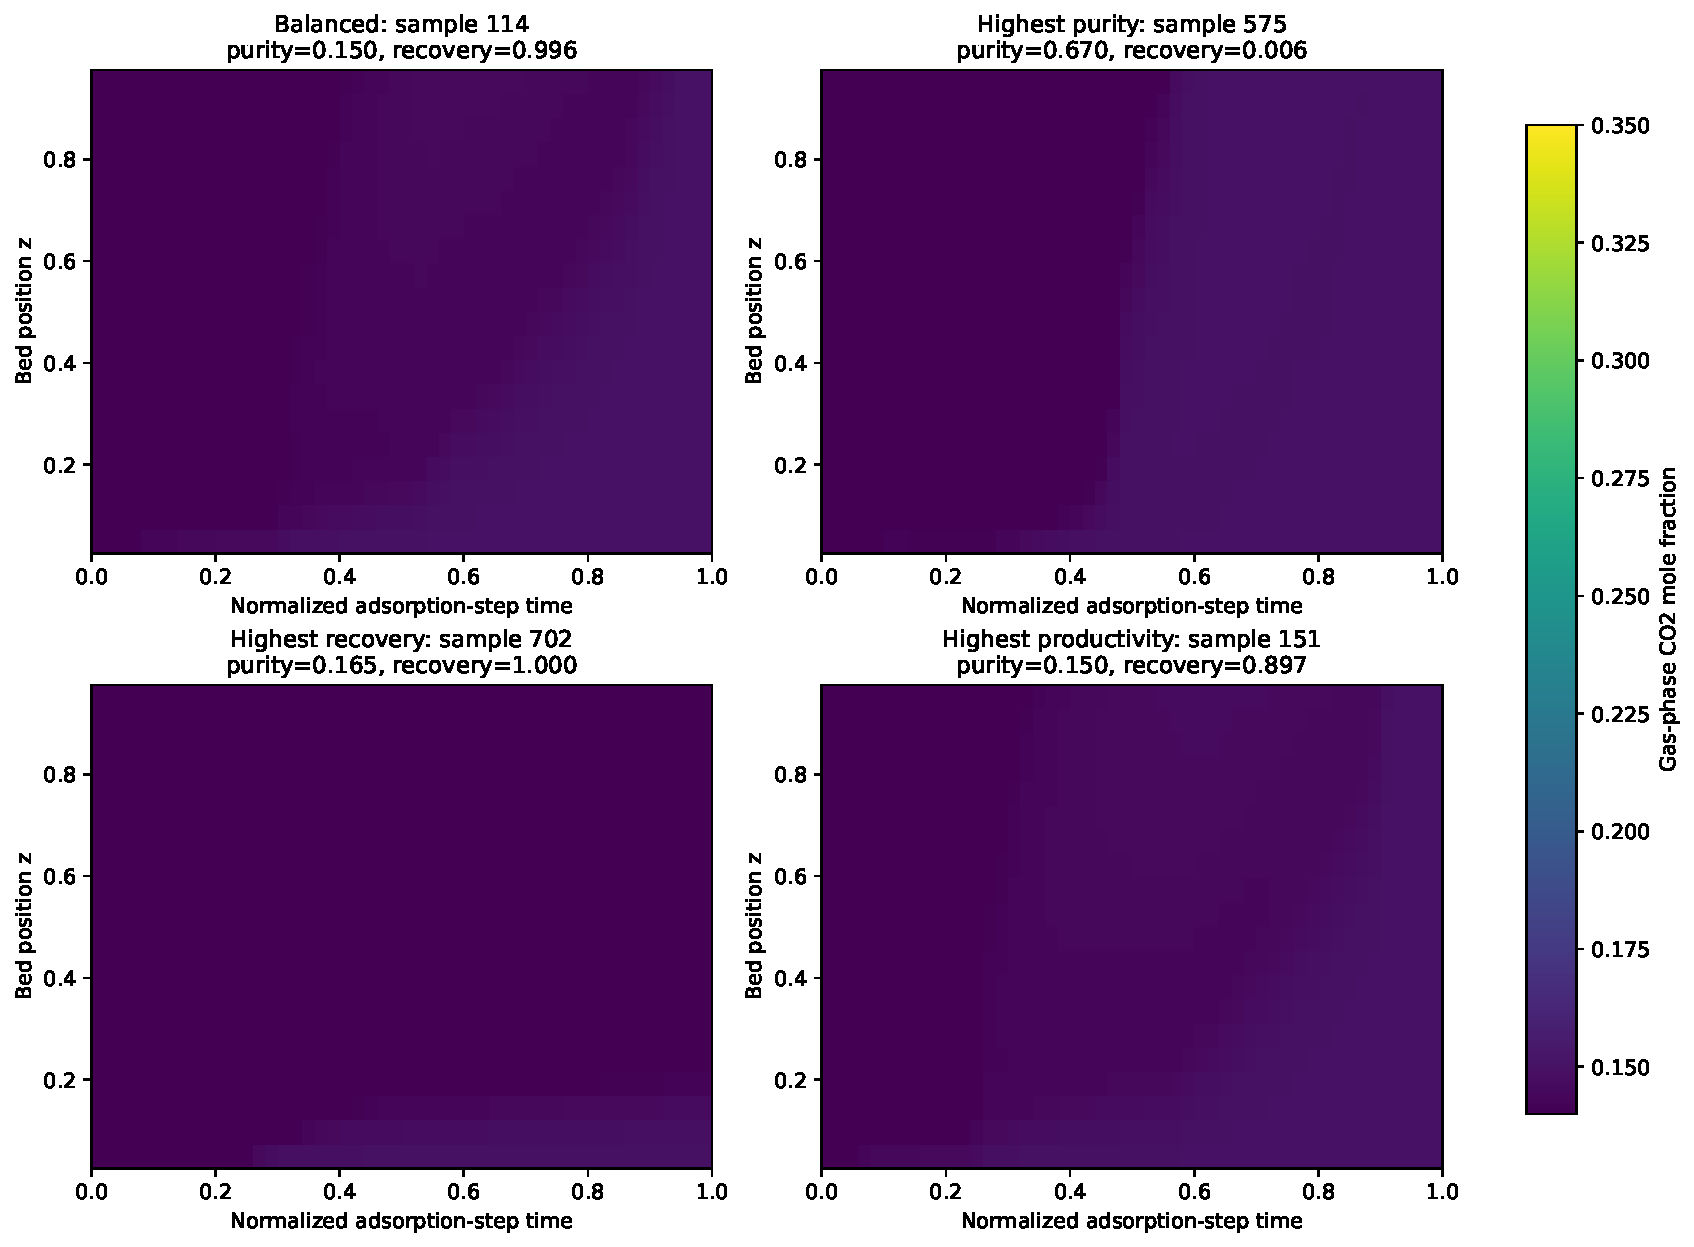
\includegraphics[width=0.92\textwidth]{figures/psa_ml/06_adsorption_profile_heatmaps.pdf}
\caption{Adsorption-step gas-phase CO$_2$ heatmaps for representative operating points.}
\end{figure}

\section{Conclusions}
This project demonstrates that ML can add measurable value after a mechanistic PSA simulation campaign. The design-only models already capture broad trends, but profile-derived features raise predictive performance and provide interpretable indicators tied to cycle physics. The main process insight is that the sampled operating space contains a severe purity--recovery tradeoff: very high purity is possible only with extremely low recovery and high energy, while balanced productivity and recovery cases remain close to feed-level purity. The resulting surrogate and classifier can be used as fast screening tools before running additional PSA simulations.

Limitations remain. The analysis is restricted to one adsorbent and one sampled operating domain. The profile features are engineered summaries rather than sequence models, so they may miss detailed transient patterns. Future work should expand the design domain, include material variables, and test sequence models or physics-informed neural networks on the raw spatiotemporal fields.

\section*{AI Use Acknowledgement}
Generative AI was used to assist with coding, figure generation, and English drafting. The simulation data, project interpretation, and final responsibility for the submitted work remain with the student.

\bibliographystyle{plain}
\bibliography{references}

\end{document}
